\documentclass[landscape]{report}
% PACKAGES %
\usepackage[english]{} % Sets the language
\usepackage[margin=2cm]{geometry} % Sets the margin size
\usepackage{fancyhdr} % Allows creation of headers
\usepackage{xcolor} % Allows the use of color in text
\usepackage{float} % Allows figures and tables to be floats
\usepackage{appendix}
\usepackage{amsmath} % Enhanced math package prepared by the American Mathematical Society
	\DeclareMathOperator{\sech}{sech} % Include sech
\usepackage{amssymb} % AMS symbols package
\usepackage{mathrsfs}% More math symbols
\usepackage{bm} % Allows you to use \bm{} to make any symbol bold
\usepackage{bbold} % Allows more bold characters
\usepackage{verbatim} % Allows you to include code snippets
\usepackage{setspace} % Allows you to change the spacing between lines at different points in the document
\usepackage{parskip} % Allows you alter the spacing between paragraphs
\usepackage{multicol} % Allows text division into multiple columns
\usepackage{units} % Allows fractions to be expressed diagonally instead of vertically
\usepackage{booktabs,multirow,multirow} % Gives extra table functionality
\usepackage{hyperref} % Allows hyperlinks in the document
\usepackage{rotating} % Allows tables to be rotated
\usepackage{graphicx} % Enhanced package for including graphics/figures
	% Set path to figure image files
	\graphicspath{ {"/Users/mitch/Documents/Cal/2_2017_Spring/COMPSCI 289A - Intro to Machine Learning/HW06/Figures/"} }
\usepackage{listings} % for including text files
	\lstset{basicstyle=\ttfamily\scriptsize,
        		  keywordstyle=\color{blue}\ttfamily,
        	  	  stringstyle=\color{red}\ttfamily,
          	  commentstyle=\color{gray}\ttfamily,
          	 }
\usepackage{tikz} % Allows the creation of diagrams
	\usetikzlibrary{shapes.geometric, arrows}
	\tikzstyle{forwardfn} = [rectangle, 
					  rounded corners,
					  minimum width=2cm, 
					  minimum height=1.5cm,
					  text centered, 
					  draw=black, 
					 ]
	\tikzstyle{backwardfn} = [rectangle, 
					      rounded corners,
					      minimum width=2cm, 
					      minimum height=1.5cm,
					      text centered, 
					      draw=white, 
					     ]
	\tikzstyle{placeholder} = [rectangle,
					      minimum width=2cm,
					      draw=white,
					      ]
	\tikzstyle{arrow} = [thick,->,>=stealth]
		
\newcommand{\tab}{\-\hspace{0.5cm}}
\newcommand{\sep}{\-\hspace{0.3cm}}
\newcommand{\ReLU}{\text{ReLU}}


\begin{document}
\thispagestyle{empty}


%%%%%%%%%%%%%%%%%%%%%%%%%%%%%%%%%% RNN Diagram %%%%%%%%%%%%%%%%%%%%%%%%%%%%%%%%%%

\section*{RNN Diagram - ReLU Activation on Hidden Layer}

The constructed neural net follows the diagram below. $x \in \mathbb{R}^{24}$, a feature vector with $(4\text{ hours} \times 6\text{ intervals}) =24 $ features corresponding to occupancies every 10 minutes for 4 hours before the current time. For clarity, shapes of the solutions are given in brackets. Subscript $j$ denotes a row index. $A^T_j$ indicates the transpose of $A_j$. 

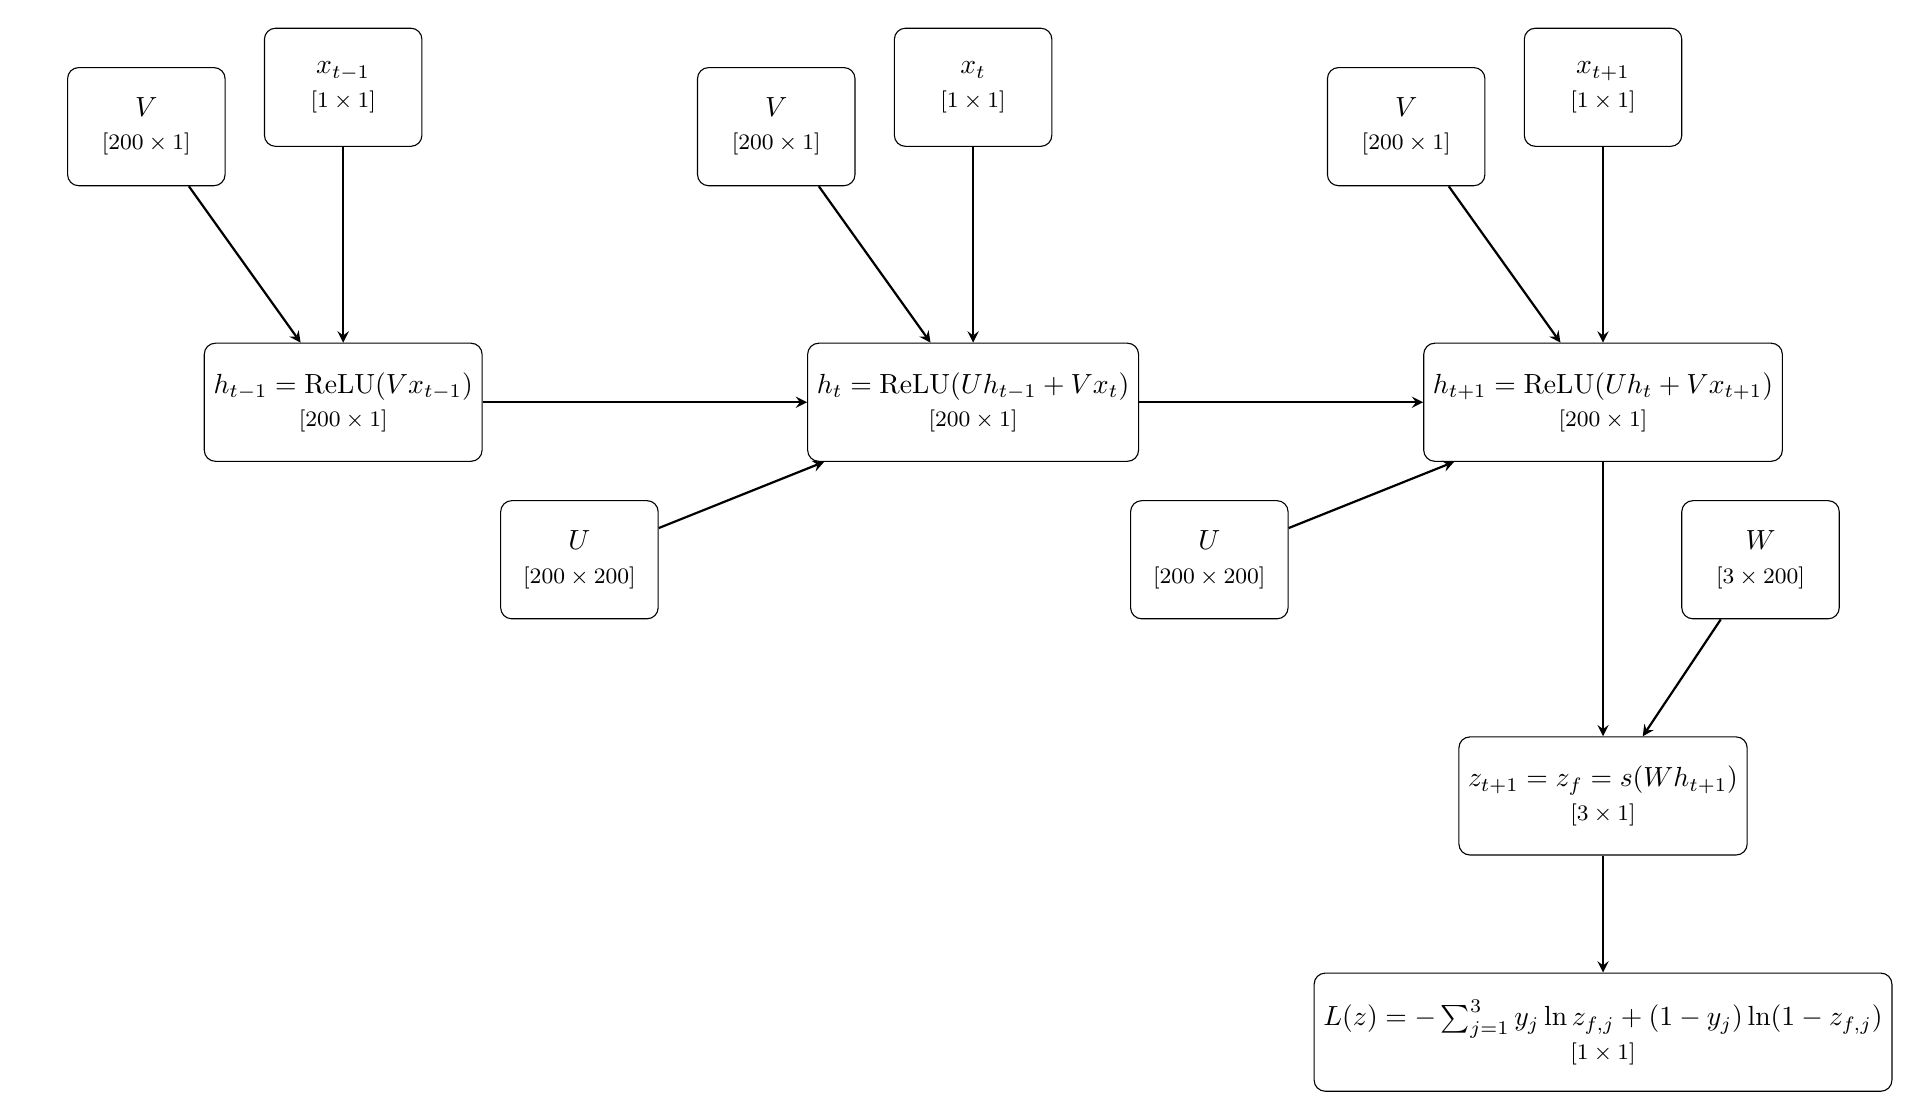
\begin{tikzpicture}[node distance=3cm]

\node (blank) [placeholder] {};
\node (x_p) [forwardfn, align=center, right of =blank] {$x_{t-1}$ \\ \footnotesize$[1\times1]$};
\node (x_c) [forwardfn, align=center, right of =x_p,xshift=5cm] {$x_{t}$ \\ \footnotesize$[1\times1]$};
\node (x_f) [forwardfn, align=center, right of =x_c,xshift=5cm] {$x_{t+1}$ \\ \footnotesize$[1\times1]$};
\node (V_p) [forwardfn, align=center, below of =blank,left of =x_p, xshift=0.5cm, yshift=2.5cm] {$V$ \\ \footnotesize$[200\times1]$};
\node (V_c) [forwardfn, align=center, below of =blank,left of =x_c, xshift=0.5cm, yshift=2.5cm] {$V$ \\ \footnotesize$[200\times1]$};
\node (V_f) [forwardfn, align=center, below of =blank,left of =x_f, xshift=0.5cm, yshift=2.5cm] {$V$ \\ \footnotesize$[200\times1]$};

\node (ReLU_p) [forwardfn, align=center, below of =x_p, yshift=-1cm] {$h_{t-1} = \ReLU(Vx_{t-1})$ \\ \footnotesize$[200\times1]$};
\node (ReLU_c) [forwardfn, align=center, below of =x_c, yshift=-1cm] {$h_{t} = \ReLU(Uh_{t-1}+Vx_{t})$ \\ \footnotesize$[200\times1]$};
\node (ReLU_f) [forwardfn, align=center, below of =x_f, yshift=-1cm] {$h_{t+1} = \ReLU(Uh_{t}+Vx_{t+1})$ \\ \footnotesize$[200\times1]$};
\node (U_c) [forwardfn, align=center, below of =ReLU_p, xshift=3cm,yshift=1cm] {$U$ \\ \footnotesize$[200\times200]$};
\node (U_f) [forwardfn, align=center, below of =ReLU_c, xshift=3cm,yshift=1cm] {$U$ \\ \footnotesize$[200\times200]$};
\node (z_f) [forwardfn, align=center, below of =ReLU_f, yshift=-2cm] {$z_{t+1} = z_f = s(Wh_{t+1})$ \\ \footnotesize$[3\times1]$};



\node (W) [forwardfn, align=center, above of =z_f, xshift=2cm] {$W$\\ \footnotesize$[3 \times 200]$};
\node (loss) [forwardfn, align=center, below of =z_f] {$ L(z) = -\sum_{j=1}^{3}{y_j \ln z_{f,j} + (1-y_j) \ln(1-z_{f,j})} $\\\footnotesize $[1\times1]$};

%\node (gradViL) [backwardfn, above of =V] {$\nabla_{V_j} L =\left(\frac{\partial L}{\partial h_j}\right) \nabla_{V_j} h_j$};
%\node (gradWjL) [backwardfn, left of =W] {$\nabla_{W_j} L = \left(\frac{\partial L}{\partial z_j}\right) \nabla_{W_j} z_j $};
%\node (gradhL) [backwardfn, right of =ReLU, yshift=-1.5cm] {$\nabla_{h} L = \sum_{j=1}^{26}{\left(\frac{\partial L}{\partial z_j}\right) \nabla_{h} z_j }$};
%\node (gradzjL) [backwardfn, right of =sigmoid, yshift=-1.4cm] {$\nabla_{z_j} L = \frac{1-y_j}{1-z_j} - \frac{y_j}{z_j} $};

\draw [arrow] (x_p) -- (ReLU_p);
\draw [arrow] (V_p) -- (ReLU_p);
\draw [arrow] (x_c) -- (ReLU_c);
\draw [arrow] (V_c) -- (ReLU_c);
\draw [arrow] (x_f) -- (ReLU_f);
\draw [arrow] (V_f) -- (ReLU_f);
\draw [arrow] (ReLU_p) -- (ReLU_c);
\draw [arrow] (ReLU_c) -- (ReLU_f);
\draw [arrow] (ReLU_f) -- (z_f);
\draw [arrow] (W) -- (z_f);
\draw [arrow] (U_c) -- (ReLU_c);
\draw [arrow] (U_f) -- (ReLU_f);


\draw [arrow] (z_f) -- (loss);

\end{tikzpicture}
\newpage
$ A_{k} = U h_{k-1} + V x_{k} $\\
\-\\

$\nabla_{V} L =$\\
$\left(\nabla_{z_f} L \right)\left( \nabla_{V} z_{t+1}\right) =$\\
$ \left(\nabla_{z_f} L \right) \left(\nabla_{h_{t+1}} z_{t+1}\right) \left( \nabla_{V} h_{t+1} \right) = $\\
$ \left( \frac{1-y_j}{1-z_j} - \frac{y_j}{z_j} \right)\left(z_j(1-z_j)W_j^T\right) \left( \nabla_{V} h_{t+1} \right) = $\\
$ \left( z_j - y_j \right)W_j^T \left( \nabla_{V} h_{t+1} \right) = $\\
$ W_j^T\left( z_j - y_j \right) \left( \nabla_{V} h_{t+1} \right) = $\\
$ W^T(z-y)\left( \nabla_{V} h_{t+1} \right) = $\\
$ W^T(z-y)\left( \nabla_{A_{t+1}} h_{t+1} \right)\left(\nabla_{V} A_{t+1}\right) =$\\
$ W^T(z-y)\left( \nabla_{A_{t+1}} h_{t+1} \right) \left(\nabla_{V} U h_t + \nabla_{V} Vx_{t+1}\right) =$\\
$ W^T(z-y)\left( \nabla_{A_{t+1}} h_{t+1} \right) \left(\nabla_{V} U h_t \right) + W^T(z-y)\left( \nabla_{A_{t+1}} h_{t+1} \right) \left(\nabla_{V} Vx_{t+1}\right) = $\\
$ W^T(z-y)\left( \nabla_{A_{t+1}} h_{t+1} \right) \left(U \nabla_{V} h_t \right) + W^T(z-y)\left( \nabla_{A_{t+1}} h_{t+1} \right) \left(I^{[200\times200]} x_{t+1}\right) = $\\
$ W^T(z-y)\left( \nabla_{A_{t+1}} h_{t+1} \right) U \left( \nabla_{A_{t}} h_{t} \right)\left(\nabla_{V} A_{t}\right) + W^T(z-y)\left( \nabla_{A_{t+1}} h_{t+1} \right) \left(I^{[200\times200]} x_{t+1}\right) = $\\
$ W^T(z-y)\left( \nabla_{A_{t+1}} h_{t+1} \right) U \left( \nabla_{A_{t}} h_{t} \right)\left(\nabla_{V} U h_{t-1} + \nabla_{V} Vx_{t}\right) + W^T(z-y)\left( \nabla_{A_{t+1}} h_{t+1} \right) \left(I^{[200\times200]} x_{t+1}\right) = $\\
$ W^T(z-y)\left( \nabla_{A_{t+1}} h_{t+1} \right) U \left( \nabla_{A_{t}} h_{t} \right)\left(\nabla_{V} U h_{t-1}\right) + W^T(z-y)\left( \nabla_{A_{t+1}} h_{t+1} \right) U \left( \nabla_{A_{t}} h_{t} \right)\left(\nabla_{V} Vx_{t}\right) + W^T(z-y)\left( \nabla_{A_{t+1}} h_{t+1} \right) \left(I^{[200\times200]} x_{t+1}\right) = $\\
$ W^T(z-y)\left( \nabla_{A_{t+1}} h_{t+1} \right) U \left( \nabla_{A_{t}} h_{t} \right) U \left(\nabla_{V} h_{t-1}\right) + W^T(z-y)\left( \nabla_{A_{t+1}} h_{t+1} \right) U \left(I^{[200\times200]} x_{t}\right)\left( \nabla_{A_{t}} h_{t} \right) + W^T(z-y) \left(I^{[200\times200]} x_{t+1}\right)\left( \nabla_{A_{t+1}} h_{t+1} \right) = $\\

$\nabla_{U} L =$\\
$\left(\nabla_{z_{t+1}} L \right)\left( \nabla_{U} z_{t+1}\right) =$\\
$ \left(\nabla_{z_{t+1}} L \right) \left(\nabla_{h_{t+1}} z_{t+1}\right) \left( \nabla_{U} h_{t+1} \right) = $\\
$ \left( \frac{1-y_j}{1-z_j} - \frac{y_j}{z_j} \right)\left(z_j(1-z_j)W_j^T\right)\left( \nabla_{U} h_{t+1} \right) = $\\
$ \left( z_j - y_j \right)W_j^T \left( \nabla_{U} h_{t+1} \right) = $\\
$ W_j^T\left( z_j - y_j \right) \left( \nabla_{U} h_{t+1} \right) = $\\
$ W^T(z-y) \left( \nabla_{U} h_{t+1} \right) = $\\
$ W^T(z-y) \left( \nabla_{A_{t+1}} h_{t+1} \right)\left(\nabla_{U} A_{t+1}\right) =$\\
$ W^T(z-y) \left( \nabla_{A_{t+1}} h_{t+1} \right)\left(\nabla_{U} U h_t \right) = $\\
$ W^T(z-y) \left( \nabla_{A_{t+1}} h_{t+1} \right)\left[U \nabla_{U} h_t + h_t \right] = $\\
$ W^T(z-y) \left( \nabla_{A_{t+1}} h_{t+1} \right)U \left( \nabla_{U} h_t \right) + W^T(z-y) \left( \nabla_{A_{t+1}} h_{t+1} \right) h_t = $\\
$ W^T(z-y) \left( \nabla_{A_{t+1}} h_{t+1} \right)U \left( \nabla_{A_{t}} h_{t} \right)\left(\nabla_{U} A_{t}\right) + W^T(z-y) \left( \nabla_{A_{t+1}} h_{t+1} \right) h_t = $\\
$ W^T(z-y) \left( \nabla_{A_{t+1}} h_{t+1} \right)U \left( \nabla_{A_{t}} h_{t} \right)\left(\nabla_{U} U h_{t-1}\right) + W^T(z-y) \left( \nabla_{A_{t+1}} h_{t+1} \right) h_t = $\\
$ W^T(z-y) \left( \nabla_{A_{t+1}} h_{t+1} \right)U \left( \nabla_{A_{t}} h_{t} \right)\left[U \nabla_{U} h_{t-1} + h_{t-1} \right] + W^T(z-y) \left( \nabla_{A_{t+1}} h_{t+1} \right) h_t = $\\
$ W^T(z-y) \left( \nabla_{A_{t+1}} h_{t+1} \right)U \left( \nabla_{A_{t}} h_{t} \right)U \left(\nabla_{U} h_{t-1}\right) + W^T(z-y) \left( \nabla_{A_{t+1}} h_{t+1} \right)U \left( \nabla_{A_{t}} h_{t} \right)h_{t-1} + W^T(z-y) \left( \nabla_{A_{t+1}} h_{t+1} \right) h_t = $\\

$\nabla_W L = $\\
$\left(\nabla_{z_f} L \right)\left(\nabla_W z_f \right) $\\
$(\nabla_{z_j} L)(\nabla_{W_j} z_j)$\\
$ \left( \frac{1-y_j}{1-z_j} - \frac{y_j}{z_j} \right) z_j(1-z_j)h_f^T$\\
$ \left(z_j - y_j \right) h_f^T$\\
$ (z-y)h_f^T $\tab\footnotesize$[3\times200]$\normalsize\\

$\nabla_{z_j} L = \frac{1-y_j}{1-z_j} - \frac{y_j}{z_j} $\\
$\nabla_{W_j} z_j = z_j(1-z_j)h^T$\tab\footnotesize$[1\times200]$\normalsize\\
$\nabla_{h} z_j = z_j(1-z_j)W_j^T$\tab\footnotesize$[201\times1]$\normalsize\\
$\nabla_{A} h = \left(\text{elementwise}\right) \begin{cases} 1, & h_j>0 \\ 0, & h_j<0 \end{cases} $\\
$\nabla_{U} h = \text{recursive expansion}$\\
$\nabla_{U} h = \text{recursive expansion}$

\-\\

\-\\

We can substitute the following expressions:\\
\tab$\nabla_{h} z_j = z_j(1-z_j)W_j^T$\tab\footnotesize$[201\times1]$\normalsize\\
\tab$\nabla_{V_j} h_j = \sech^2(V_jx)x^T $\tab\footnotesize$[1\times785]$\normalsize\\

We can also use backpropagation to show:\\
\tab$\nabla_{W_j} L = \left(\frac{1-y_j}{1-z_j} - \frac{y_j}{z_j}\right)\left(z_j(1-z_j) h^T\right)$\tab\footnotesize$[1\times201]$\normalsize\\
\tab$\nabla_{h} L = \sum_{j=1}^{26}{\left(\frac{1-y_j}{1-z_j} - \frac{y_j}{z_j}\right)\left(z_j(1-z_j)W_j^T\right)}$\tab\footnotesize$[201\times1]$\normalsize\\
\tab$\nabla_{V_j} L = \left(\nabla_{h} L\right)_j \sech^2(V_jx)x^T $\tab\footnotesize$[1\times785]$\normalsize\\

To enhance calculation efficiency, we can reduce some of these equations into matrices. First, let $\mathcal{Q}$ be the matrix
$$\mathcal{Q} = \begin{bmatrix}
z_1(1-z_1)\left(\frac{1-y_1}{1-z_1} - \frac{y_1}{z_1}\right)\\
z_2(1-z_2)\left(\frac{1-y_2}{1-z_2} - \frac{y_2}{z_2}\right)\\
\vdots \\
z_{26}(1-z_{26})\left(\frac{1-y_{26}}{1-z_{26}} - \frac{y_{26}}{z_{26}}\right)\\
\end{bmatrix} = \begin{bmatrix}
z_1 - y_1\\
z_2 - y_2 \\
\vdots \\
z_{26} - y_{26} \\
\end{bmatrix}$$

With this, we can reexpress the above equations.\\
(1) \\
\tab$\nabla_{W_j} L = \mathcal{Q}_j h^T $\tab\footnotesize$[1\times201]$\normalsize\\
\tab or
$$ \nabla_{W} L = \begin{bmatrix}
\mathcal{Q}_1 h^T \\
\mathcal{Q}_2 h^T \\
\vdots \\
\mathcal{Q}_{26} h^T \\
\end{bmatrix} = \mathcal{Q}h^T = \mathcal{Q} \otimes h \text{\tab\footnotesize$[26\times201]$\normalsize} $$

(2)\\
\tab$\nabla_{h} L = \sum_{j=1}^{26}{\mathcal{Q}_j W_j^T}$\tab\footnotesize$[201\times1]$\normalsize\\
\tab or
$$ \nabla_{h} L = \begin{bmatrix}
\mathcal{Q}_1 W_1^T + \mathcal{Q}_2 W_2^T + ... + \mathcal{Q}_{26} W_{26}^T\\
\end{bmatrix} $$
$$ \nabla_{h} L = \begin{bmatrix}
W_1^T \mathcal{Q}_1 + W_2^T \mathcal{Q}_2 + ... + W_{26}^T \mathcal{Q}_{26}\\
\end{bmatrix} $$
$$ \nabla_{h} L = \begin{bmatrix}
W_1^T & W_2^T & \hdots & W_{26}^T \\
\end{bmatrix}\begin{bmatrix}
\mathcal{Q}_1 \\
\mathcal{Q}_2 \\
\vdots \\
\mathcal{Q}_{26} \\
\end{bmatrix} = W^T \mathcal{Q} \text{\tab\footnotesize$[201\times1]$\normalsize} $$

(3)\\
Additionally, let
$$ \mathcal{S} = \begin{bmatrix}
\sech^2(V_1 x) \\
\sech^2(V_2 x) \\
\vdots \\
\sech^2(V_{200} x)\\
\end{bmatrix} = \sech^2(Vx) $$
Then, $\nabla_{V_j} L = (W^T \mathcal{Q})_j \sech^2(V_jx)x^T $\tab\footnotesize$[1\times785]$\normalsize\\
\tab or
$$ \nabla_{V} L = \begin{bmatrix}
(W^T \mathcal{Q})_1 \sech^2(V_1 x)x^T \\
(W^T \mathcal{Q})_2 \sech^2(V_2 x)x^T \\
\vdots \\
(W^T \mathcal{Q})_{200} \sech^2(V_{200}x)x^T \\
\end{bmatrix} = \begin{bmatrix}
(W^T \mathcal{Q})_1 \sech^2(V_1 x) \\
(W^T \mathcal{Q})_2 \sech^2(V_2 x) \\
\vdots \\
(W^T \mathcal{Q})_{200} \sech^2(V_{200}x)
\end{bmatrix} x^T $$
$$\nabla_{V} L = \left(\begin{bmatrix}
(W^T \mathcal{Q})_1 \\
(W^T \mathcal{Q})_2 \\
\vdots \\
(W^T \mathcal{Q})_{200} \\
\end{bmatrix} \circ \begin{bmatrix}
\sech^2(V_1 x) \\
\sech^2(V_2 x) \\
\vdots \\
\sech^2(V_{200}x)
\end{bmatrix}\right) x^T = (W^T \mathcal{Q}) \circ \mathcal{S} x^T $$

\newpage
Since we are updating our matrices $V$ and $W$ using stochastic gradient descent, we repeat the following process:

\tab $V,W \leftarrow$ weight matrices initialized randomly from normal distribution with mean $\mu=0$ and $
\sigma^2 = (...)$\\
\tab while (continue = True or $L(z) > 0$) \\
\tab \tab \tab Forward calculation [ $h = \tanh(Vx)$\sep$\rightarrow$\sep$z = s(Wh)$\sep$\rightarrow$\sep$L(z)$ ]\\
\tab \tab \tab Backward calculation to return $\nabla_V L$ and $\nabla_W L$\\
\tab \tab \tab $V \leftarrow V - \epsilon \nabla_V L)$ \\
\tab \tab \tab $W \leftarrow W - \epsilon \nabla_W L$ \\
\tab return $V,W$ \\

where, using our derived equations from above, the update rules are more specifically\\
\tab \tab \tab \tab $V \leftarrow V - \epsilon(W^T \mathcal{Q}) \circ \mathcal{S} x^T $\\
\tab \tab \tab \tab $ W \leftarrow W - \epsilon(\mathcal{Q} \otimes h). $

$ h = \ReLU(Uh_{t-1} + V x_t)$\\
$ \partial h/ \partial h_{t-1} = \text{RLD}(Uh_{t-1} + V x_t)U^T $\\
$ \partial h/ \partial V = \text{RLD}(Uh_{t-1} + V x_t)(\partial (U h_{t-1})/ \partial V + \partial (Vx_t)/ \partial V )= \text{RLD}(Uh_{t-1} + V x_t)(U^T\frac{\partial h_{t-1}}{\partial h_{t-2}}(...)\frac{\partial h_{0}}{\partial V} + I x_t  ) $\\
$\partial h_0/ \partial V = $\\
$ \partial h/ \partial U = \text{RLD}(Uh_{t-1} + V x_t)(\partial (U h_{t-1})/ \partial U + \partial (Vx_t)/ \partial U )= \text{RLD}(Uh_{t-1} + V x_t)(U^T\frac{\partial h_{t-1}}{\partial h_{t-2}}(...)\frac{\partial h_{0}}{\partial V} + I x_t  ) $\\



$ y = \sin(Ax)$\\
$ \partial y/\partial x = \frac{\partial (Ax)}{\partial x}\cos(Ax) = A^T \cos(Ax) $\\
$[200\times200] = [200\times1] (...)$

\end{document}




